\chapter{Machine Learning Models}

\section{Introduction}
As explained in dept in the methodology chapter, the biometric data collected through the watches generated a total of 6 independent variables:

\begin{itemize}
    \item Heart Rate Maximum \textit{bm\_HR\_max}
    \item Heart Rate Average \textit{bm\_HR\_avg}
    \item Heart Rate Variability \textit{bm\_HR\_var}
    \item Activity Steps \textit{bm\_act\_steps}
    \item Sleep \textit{bm\_sleep}
\end{itemize}

The dependent variables that were collected through the gaming tests are:

\begin{itemize}
    \item Fine Motor Tracking Time \textit{fm\_avg\_trk\_time}
    \item Fine Motor Accuracy \textit{fm\_accuracy}
    \item Visual Average Response Time \textit{vx\_avg\_res\_time}
    \item Visual Shot Accuracy \textit{vx\_shot\_accuracy}
    \item Visual Target Accuracy \textit{vx\_trg\_accuracy}
    \item Audio Average Response Time \textit{au\_avg\_res\_time}
\end{itemize}

The goal based on the research question was to find the correlation between the independent and dependent variables. When approaching a machine learning problem, one of the fundamental
considerations is wheter the problem is a regression or classification problem. 

\subsection*{Classification Problem}
Classification is used when the dependent variable is categorical, meaning it can take one of a limited number of values. Examples includes predicting whether an email is spam or not,
whether a patient has a disease or not, whether a customer will buy a product or not. 

\subsection*{Regression Problem}
Regression is used when the dependent variable is continuous and numerical, meaning it can take any value within a range. Examples includes predicting house prices, stock prices, 
temperature. In this project, the dependent variables are continuous and numerical, making it a regression problem. The goal was to predict the dependent variables based on the biometric
data collected from the watches. 

\section{Data Exploration}
The first step in the machine learning process was to explore the dataset. The dataset was loaded into a pandas dataframe and the first 5 rows were displayed to get an overview of the
data. The shape of the dataset was checked to see the number of rows and columns. The data types of the columns were checked to ensure that the data types were correct. The summary
statistics of the dataset were checked to see the mean, median, standard deviation, minimum and maximum values of the dataset. The correlation between the independent and dependent
variables were checked to see if there was any correlation between the variables. The correlation was visualized using a heatmap \ref{fig:correlation_heatmap} to see the correlation 
between the variables.

\begin{figure}[H]
    \centering
    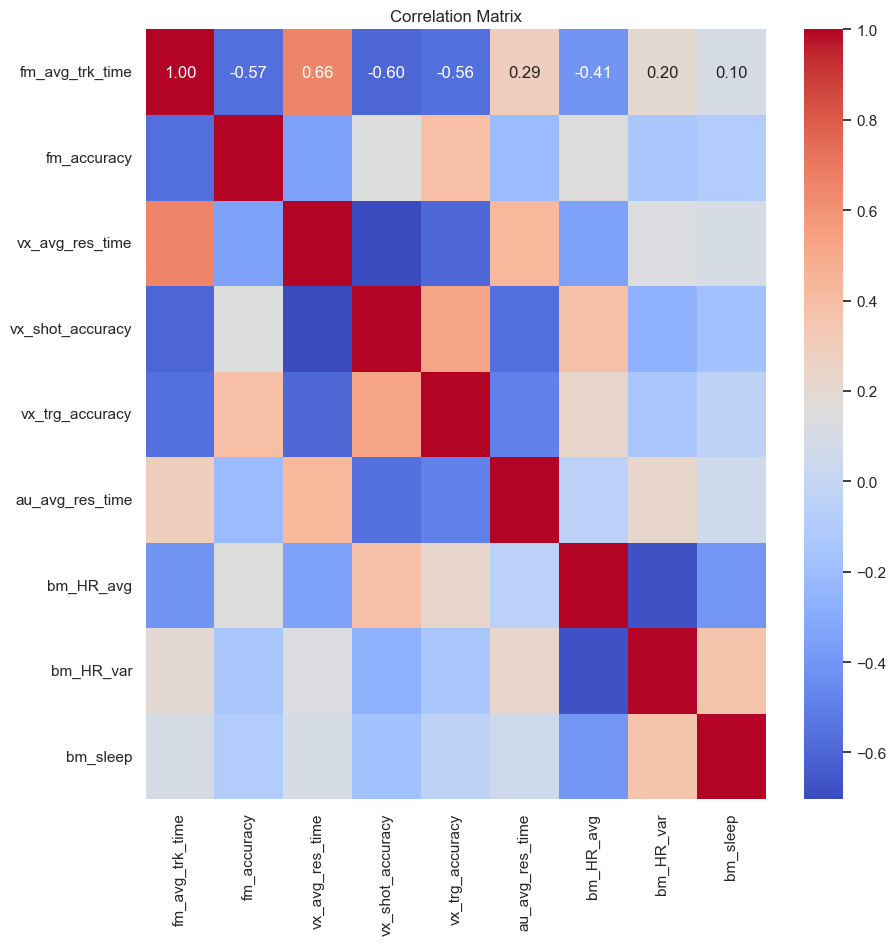
\includegraphics[width=1\textwidth]{images/correlation.png}
    \caption{Correlation Heatmap}
    \label{fig:correlation_heatmap}
\end{figure}

The correlation heatmap shows the correlation between the independent and dependent variables. The correlation values range from -1 to 1. A value of 1 indicates 
a strong positive correlation, a value of -1 indicates a strong negative correlation and a value of 0 indicates no correlation. The correlation heatmap shows 
the following correlations between the dependent and the independent variables:

\subsubsection*{Heart Rate Average (\textit{bm\_HR\_avg})}
\begin{itemize}
    \item Fine Motor Tracking Time (\textit{fm\_avg\_trk\_time}): A negative correlation of \\ -0.41 suggests that as the average heart rate increases, the fine motor
    tracking time tasks decreases, indicating that individuals with faster heart rates tend to complete fine motor tasks a bit quicker.
    \item Fine Motor Accuracy (\textit{fm\_accuracy}): A positive correlation of 0.16 indicates a weak relationship suggesting that a higher heart rate average might be very 
    slightly associated with higher fine motor accuracy. It shows that there is a small tendency for individuals with a higher heart rate to be slightly more precise
    in tasks that need fine motor skills.
    \item Visual Average Response Time (\textit{vx\_avg\_res\_time}): A negative correlation of -0.35 suggests a moderate relationship where a higher average heart rate
    is associated with faster response times. It indicates that individuals with higher heart rates also tend to react faster to visual things.
    \item Visual Shot Accuracy (\textit{vx\_shot\_accuracy}): A positive correlation of 0.38 indicates a moderate relationship, suggesting that individuals with higher heart
    rate might have a better accuracy in shooting tasks.
    \item Visual Target Accuracy (\textit{vx\_trg\_accuracy}): A positive correlation of 0.22 indicates a weak relationship, suggesting that higher heart rates averages might
    be associated with slightly better visual target accuracy.
    \item Audio Average Response Time (\textit{au\_avg\_res\_time}): A very weak negative correlation of -0.05 suggest almost no relationship between average heart rate
    and audio response time. It indicates there is no real connection between heart rate and how quickly the individuals responds to sounds.
\end{itemize}

\subsubsection*{Hear Rate Variability (\textit{bm\_HR\_var})}

\begin{itemize}
    \item Fine Motor Tracking Time (\textit{fm\_avg\_trk\_time}): A positive correlation of 0.20 suggests a weak association where greater heart rate variability 
    might be associated with slightly longer fine motor tracking time tasks.
    
    \item Fine Motor Accuracy (\textit{fm\_accuracy}): A negative correlation of -0.14 suggest a very weak inverse relationship, where higher heart rate variability
    could be slightly associated with a decrease in fine motor accuracy.
    
    \item Visual Average Response Time (\textit{vx\_avg\_res\_time}): A positive correlation of 0.13 indicates very weak relationship, with slightly tendency for
    higher heart rate variability to be associated with longer visual response times. 
    
    \item Visual Shot Accuracy (\textit{vx\_shot\_accuracy}): A negative correlation of -0.27 indicates a weak to moderate inverse relationship, suggesting that
    higher rate variability might be associated with a decrease in visual shot accuracy. It suggests that individuals with higher heart rate variability might 
    have a lower accuracy in shooting tasks.
    
    \item Visual Target Accuracy (\textit{vx\_trg\_accuracy}): A negative correlation of -0.14 indicates a weak inverse relationship, suggesting that higher heart 
    variability could slightly correlate with lower visual target accuracy. It suggests that those with more variation in their heart rate might not be quite as good 
    at tasks that involve quickly identifying and selecting targets.
    
    \item Audio Average Response Time (\textit{au\_avg\_res\_time}): A positive correlation of 0.22 suggests a weak relationship, indicating that higher heart rate
    variability might be associated with slightly longer audio response times.
    
\end{itemize}


\subsubsection*{Sleep (\textit{bm\_sleep})}

\begin{itemize}
    \item Fine Motor Tracking Time (\textit{fm\_avg\_trk\_time}): 
    
    \item Fine Motor Accuracy (\textit{fm\_accuracy}): 
    
    \item Visual Average Response Time (\textit{vx\_avg\_res\_time}): 
    
    \item Visual Shot Accuracy (\textit{vx\_shot\_accuracy}): 
    
    \item Visual Target Accuracy (\textit{vx\_trg\_accuracy}): 
    
    \item Audio Average Response Time (\textit{au\_avg\_res\_time}):
    
\end{itemize}



\section{Data Pre-processing}
To have the dataset suitable for the machine learning models, the data was pre-processed. It was found that were many null values that needed to be handled, 
it was removed from the dataset as it was not possible to impute the values. The \section{Activity Steps} and \section{Heart Rate Maximum} were found to have
outliers that were removed from the dataset. The data was then scaled using StandardScaler from the sklearn library. This was done to ensure that all the features
contribute equally to the result.
The columns \textit{\_id}, \textit{\_date} and \textit{\_user} were removed from the dataset as they were not needed for the machine learning models.


\section{Model Selection and Evaluation}
Various machine learning models were explored to address the research question and predict the dependent variables based on the collected biometric and gaming test. Each team member
focused on developing and evaluating a model to achieve the best predictive performance. 


\section{Classical ML Regression Model}
The first model that was explored was the classical machine learning regression model. The model was trained using the training dataset and evaluated using the testing dataset. 
The model was evaluated using the mean squared error. The model was trained using the following algorithms:

\begin{itemize}
    \item Linear Regression: Chose as a baseline for its simplicity and interpretability, assuming a linear relationship between the dependent and independent variables.
    \item Random Forest Regressor: Chose for its ability to handle non-linear relationships and its robustness to overfitting. 
    \item Support Vector Regressor: Selected for its ability to handle high-dimensional data and capability to find complex patterns by mapping input data into a higher-dimensional feature space.
    \item K-Nearest Neighbours Regressor: Chose for its simplicity and effectiveness in regression tasks, making predictions based on the average of the k-nearest neighbours in the feature space.
\end{itemize}

Each model was trained on pre-processed data and evaluated using the standard regression performance metric mean squared error (MSE). The best performing model for each variable was 
identified utilized for further analysis.




\section{Neural Network Regression Model}



